
\documentclass{article}
\usepackage[left=1cm,right=1cm]{geometry}
\usepackage{float}

\usepackage[htt]{hyphenat}
\usepackage{graphicx}
\usepackage{courier}



\begin{document}

\title{Atomic oven testing guide}
\date{\today}

\maketitle

\section{Wiring}

\begin{figure}[H]
    \center
    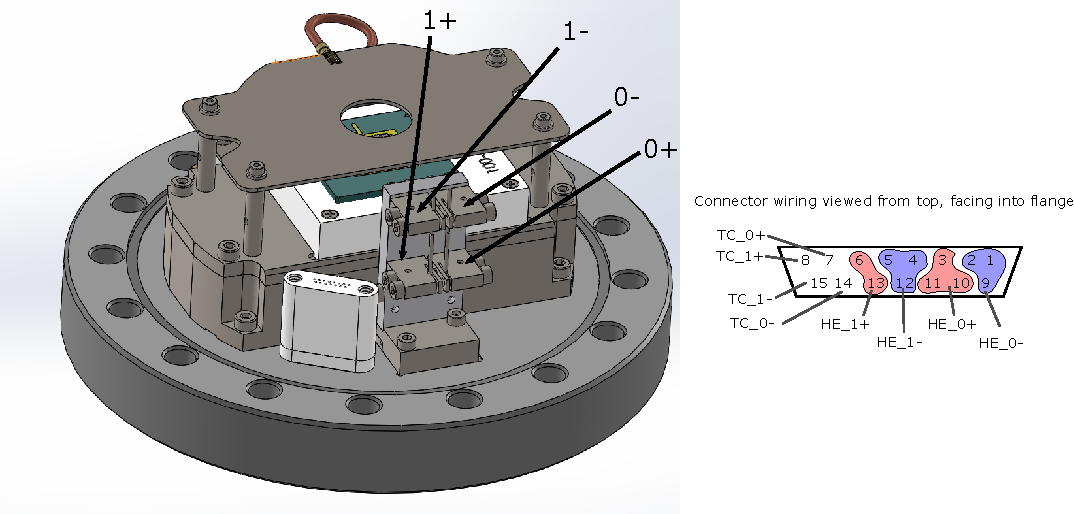
\includegraphics[scale=1]{figures/baseflange_wiring.pdf} 
    \caption{Wiring of in vacuum oven connector}
    \label{fig:baseflange_wiring}
\end{figure}

\section{Temperature readout}
Run the script in \texttt{oven\_test\_scripts/temperature\_readout} to print out temperature measurements in real time. Touch the thermocouples on each tube one after the other to check that the temperature reading changes.

\section{Low power testing}
Measure the current, voltage, and temperature characteristics of the oven at a low/safe power. Run the script in \texttt{oven\_test\_scripts/low\_power\_heating} and enter the channel of oven to be tested. Use the plotter script to make the graph, and the output should look like figure \ref{fig:low_power_heating}.
This measurement determines that everything is connected correctly, the restance of the oven and wiring, and the polarity of the thermocouple connection.

\begin{figure}
    \center
    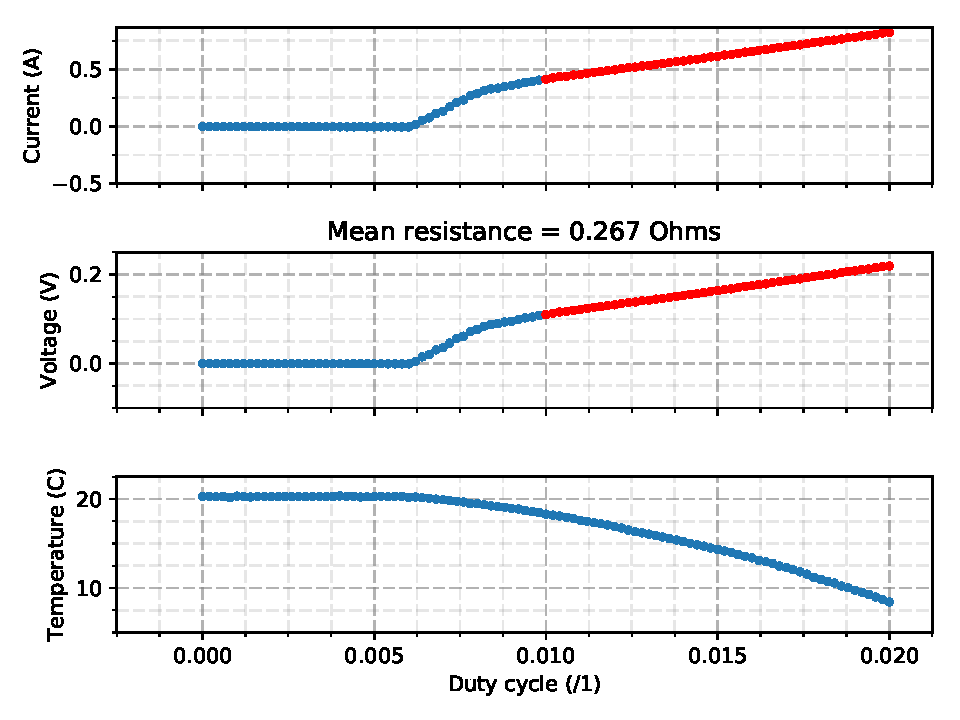
\includegraphics[scale=1]{figures/current_vs_duty_0.pdf} 
    \caption{Example data for low\_power\_heating test}
    \label{fig:low_power_heating}
\end{figure}




\end{document}

